\documentclass[letterpaper,9pt,twocolumn,twoside,]{pinp}

%% Some pieces required from the pandoc template
\providecommand{\tightlist}{%
  \setlength{\itemsep}{0pt}\setlength{\parskip}{0pt}}

% Use the lineno option to display guide line numbers if required.
% Note that the use of elements such as single-column equations
% may affect the guide line number alignment.

\usepackage[T1]{fontenc}
\usepackage[utf8]{inputenc}

% pinp change: the geometry package layout settings need to be set here, not in pinp.cls
\geometry{layoutsize={0.95588\paperwidth,0.98864\paperheight},%
  layouthoffset=0.02206\paperwidth, layoutvoffset=0.00568\paperheight}

\definecolor{pinpblue}{HTML}{185FAF}  % imagecolorpicker on blue for new R logo
\definecolor{pnasbluetext}{RGB}{0,101,165} % default in pinp.cls


\usepackage{booktabs}
\usepackage{longtable}
\usepackage{array}
\usepackage{multirow}
\usepackage{wrapfig}
\usepackage{float}
\usepackage{colortbl}
\usepackage{pdflscape}
\usepackage{tabu}
\usepackage{threeparttable}
\usepackage{threeparttablex}
\usepackage[normalem]{ulem}
\usepackage{makecell}
\usepackage{xcolor}

\title{Report Title}

\author[a]{Charley Johnson}
\author[b]{Chengxi Duan}
\author[c]{Fiona Li}
\author[d]{Hussain Karimi}
\author[e]{Imane Lattab}
\author[f]{Kunlei Zhang}
\author[g]{Oscar Lo Lu}
\author[h]{Tingzhao Dai}

  \affil[a]{}
  \affil[b]{}
  \affil[c]{}
  \affil[d]{}
  \affil[e]{}
  \affil[f]{}
  \affil[g]{}
  \affil[h]{}

\setcounter{secnumdepth}{0}

% Please give the surname of the lead author for the running footer
\leadauthor{}

% Keywords are not mandatory, but authors are strongly encouraged to provide them. If provided, please include two to five keywords, separated by the pipe symbol, e.g:
 \keywords{  enso |  great barrier reef |  gbr |  ocean temperature  }  

\begin{abstract}
executive summary
\end{abstract}

\dates{This version was compiled on \today} 


% initially we use doi so keep for backwards compatibility
% new name is doi_footer
\doifooter{\url{https://github.com/DipsyCdua/reef}}

\pinpfootercontents{Reef03 MARS/DATA3888 2025, The University of Sydney}

\begin{document}

% Optional adjustment to line up main text (after abstract) of first page with line numbers, when using both lineno and twocolumn options.
% You should only change this length when you've finalised the article contents.
\verticaladjustment{-2pt}

\maketitle
\thispagestyle{firststyle}
\ifthenelse{\boolean{shortarticle}}{\ifthenelse{\boolean{singlecolumn}}{\abscontentformatted}{\abscontent}}{}

% If your first paragraph (i.e. with the \dropcap) contains a list environment (quote, quotation, theorem, definition, enumerate, itemize...), the line after the list may have some extra indentation. If this is the case, add \parshape=0 to the end of the list environment.


\section{Formatting stuff}\label{formatting-stuff}

if (Fabricius, 2000), use \citep{fabricius2000biodiversity}

if (Kayanne, 2016), use \citep{kayanne2016validation}

(refer to \textbf{Appendix Fig.x.} for \textless\textgreater)

(refer to \textbf{Fig.x.})

\#\newpage

\section{Introduction}\label{introduction}

\section{Methods}\label{methods}

\section{Results}\label{results}

\begin{center}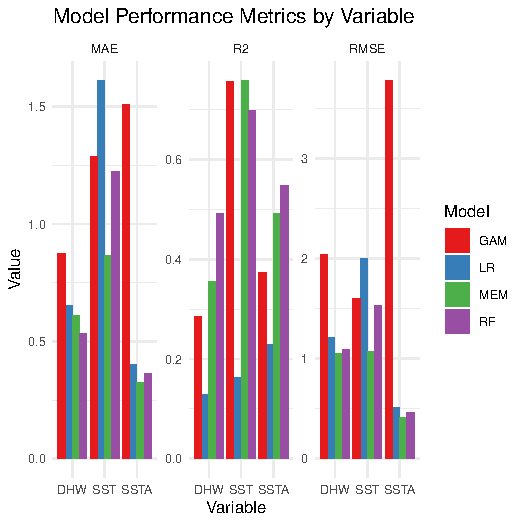
\includegraphics[width=1\linewidth,height=200px]{Reef03_FinalReport_files/figure-latex/unnamed-chunk-2-1} \end{center}

\section{Discussion}\label{discussion}

\section{Contributions}\label{contributions}

\subparagraph{Charley Johnson}\label{charley-johnson}

\subparagraph{Chengxi Duan}\label{chengxi-duan}

\subparagraph{Fiona Li}\label{fiona-li}

Finding and collating scientific literature over the semester to help
develop the research question. Editing and formatting both the report
and the presentation slides/script. Presented the introduction,
background and aims for the presentation. Worked on the executive
summary, background and aims. Assisted Oscar, Charley and Imane with the
discussion.

\subparagraph{Hussain Karimi}\label{hussain-karimi}

\subparagraph{Imane Lattab}\label{imane-lattab}

\subparagraph{Kunlei Zhang}\label{kunlei-zhang}

\subparagraph{Oscar Lo Lu}\label{oscar-lo-lu}

\subparagraph{Tingzhao Dai}\label{tingzhao-dai}

\newpage

\section{Appendix}\label{appendix}

\subsubsection{Appendix: V: Linear Regression Assumption
Checking}\label{appendix-v-linear-regression-assumption-checking}

\begin{center}
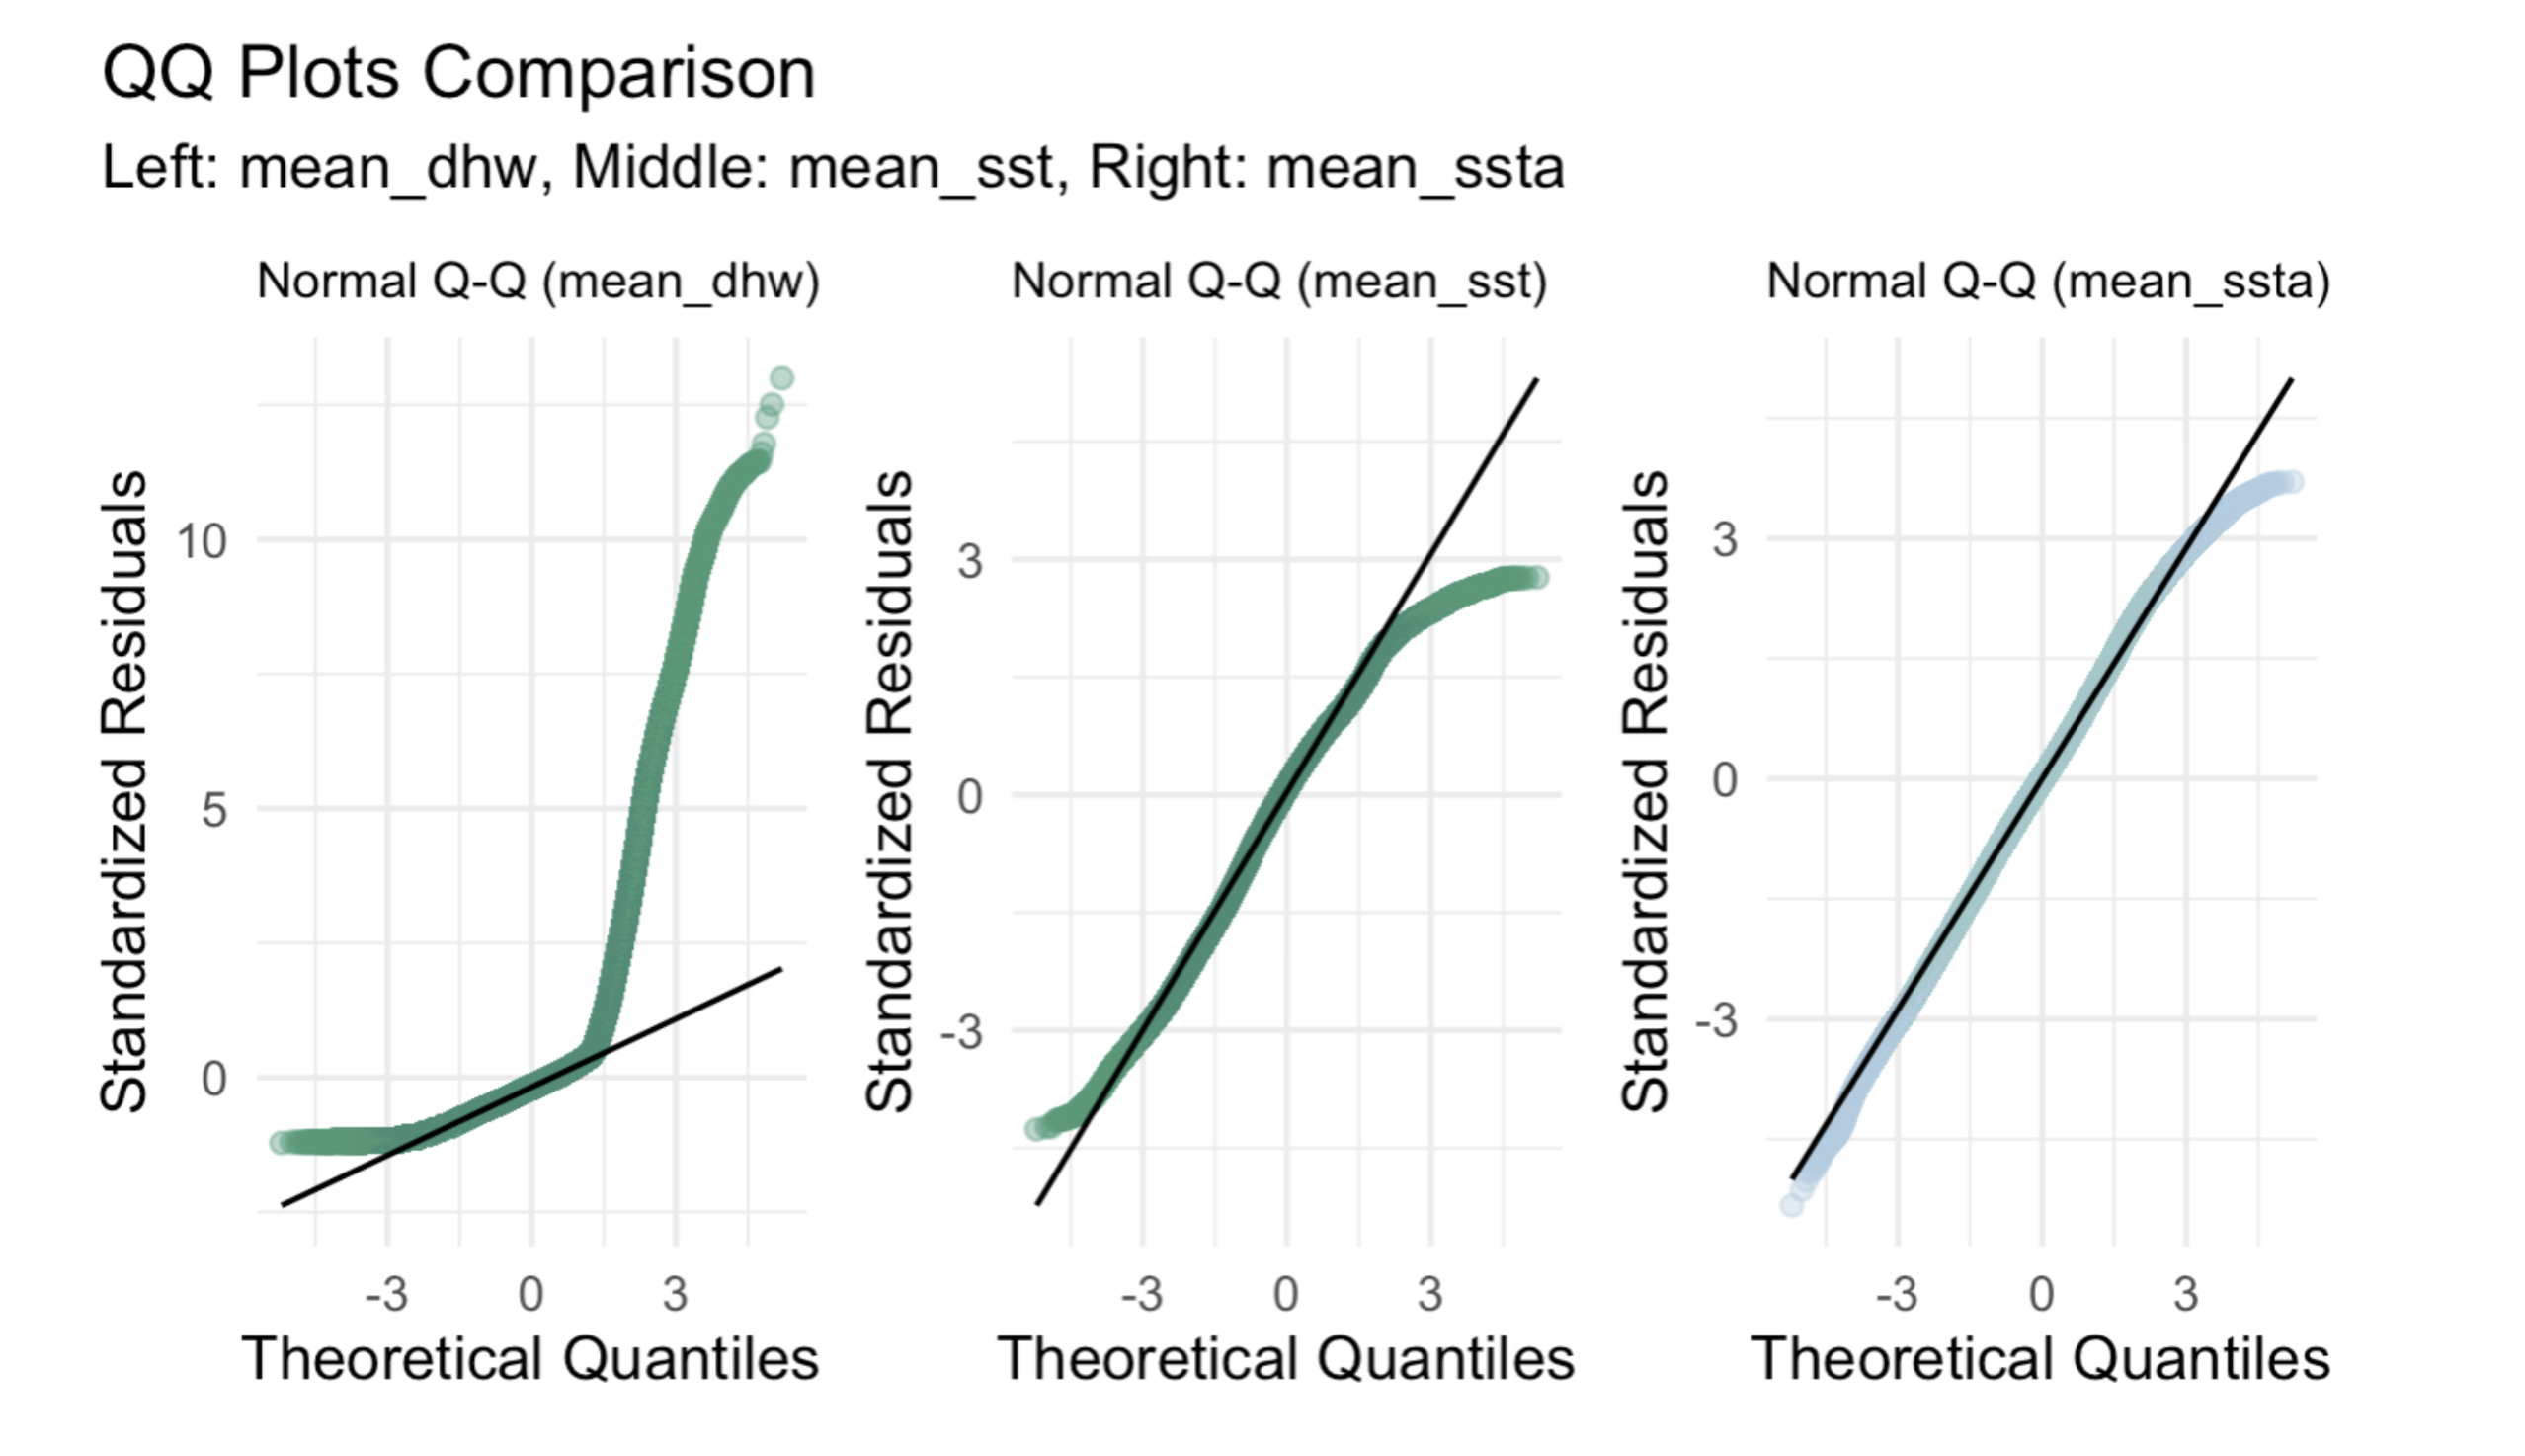
\includegraphics[width=0.5\textwidth]{report_images/lr_qqplots.png}
\end{center}

\begin{center}
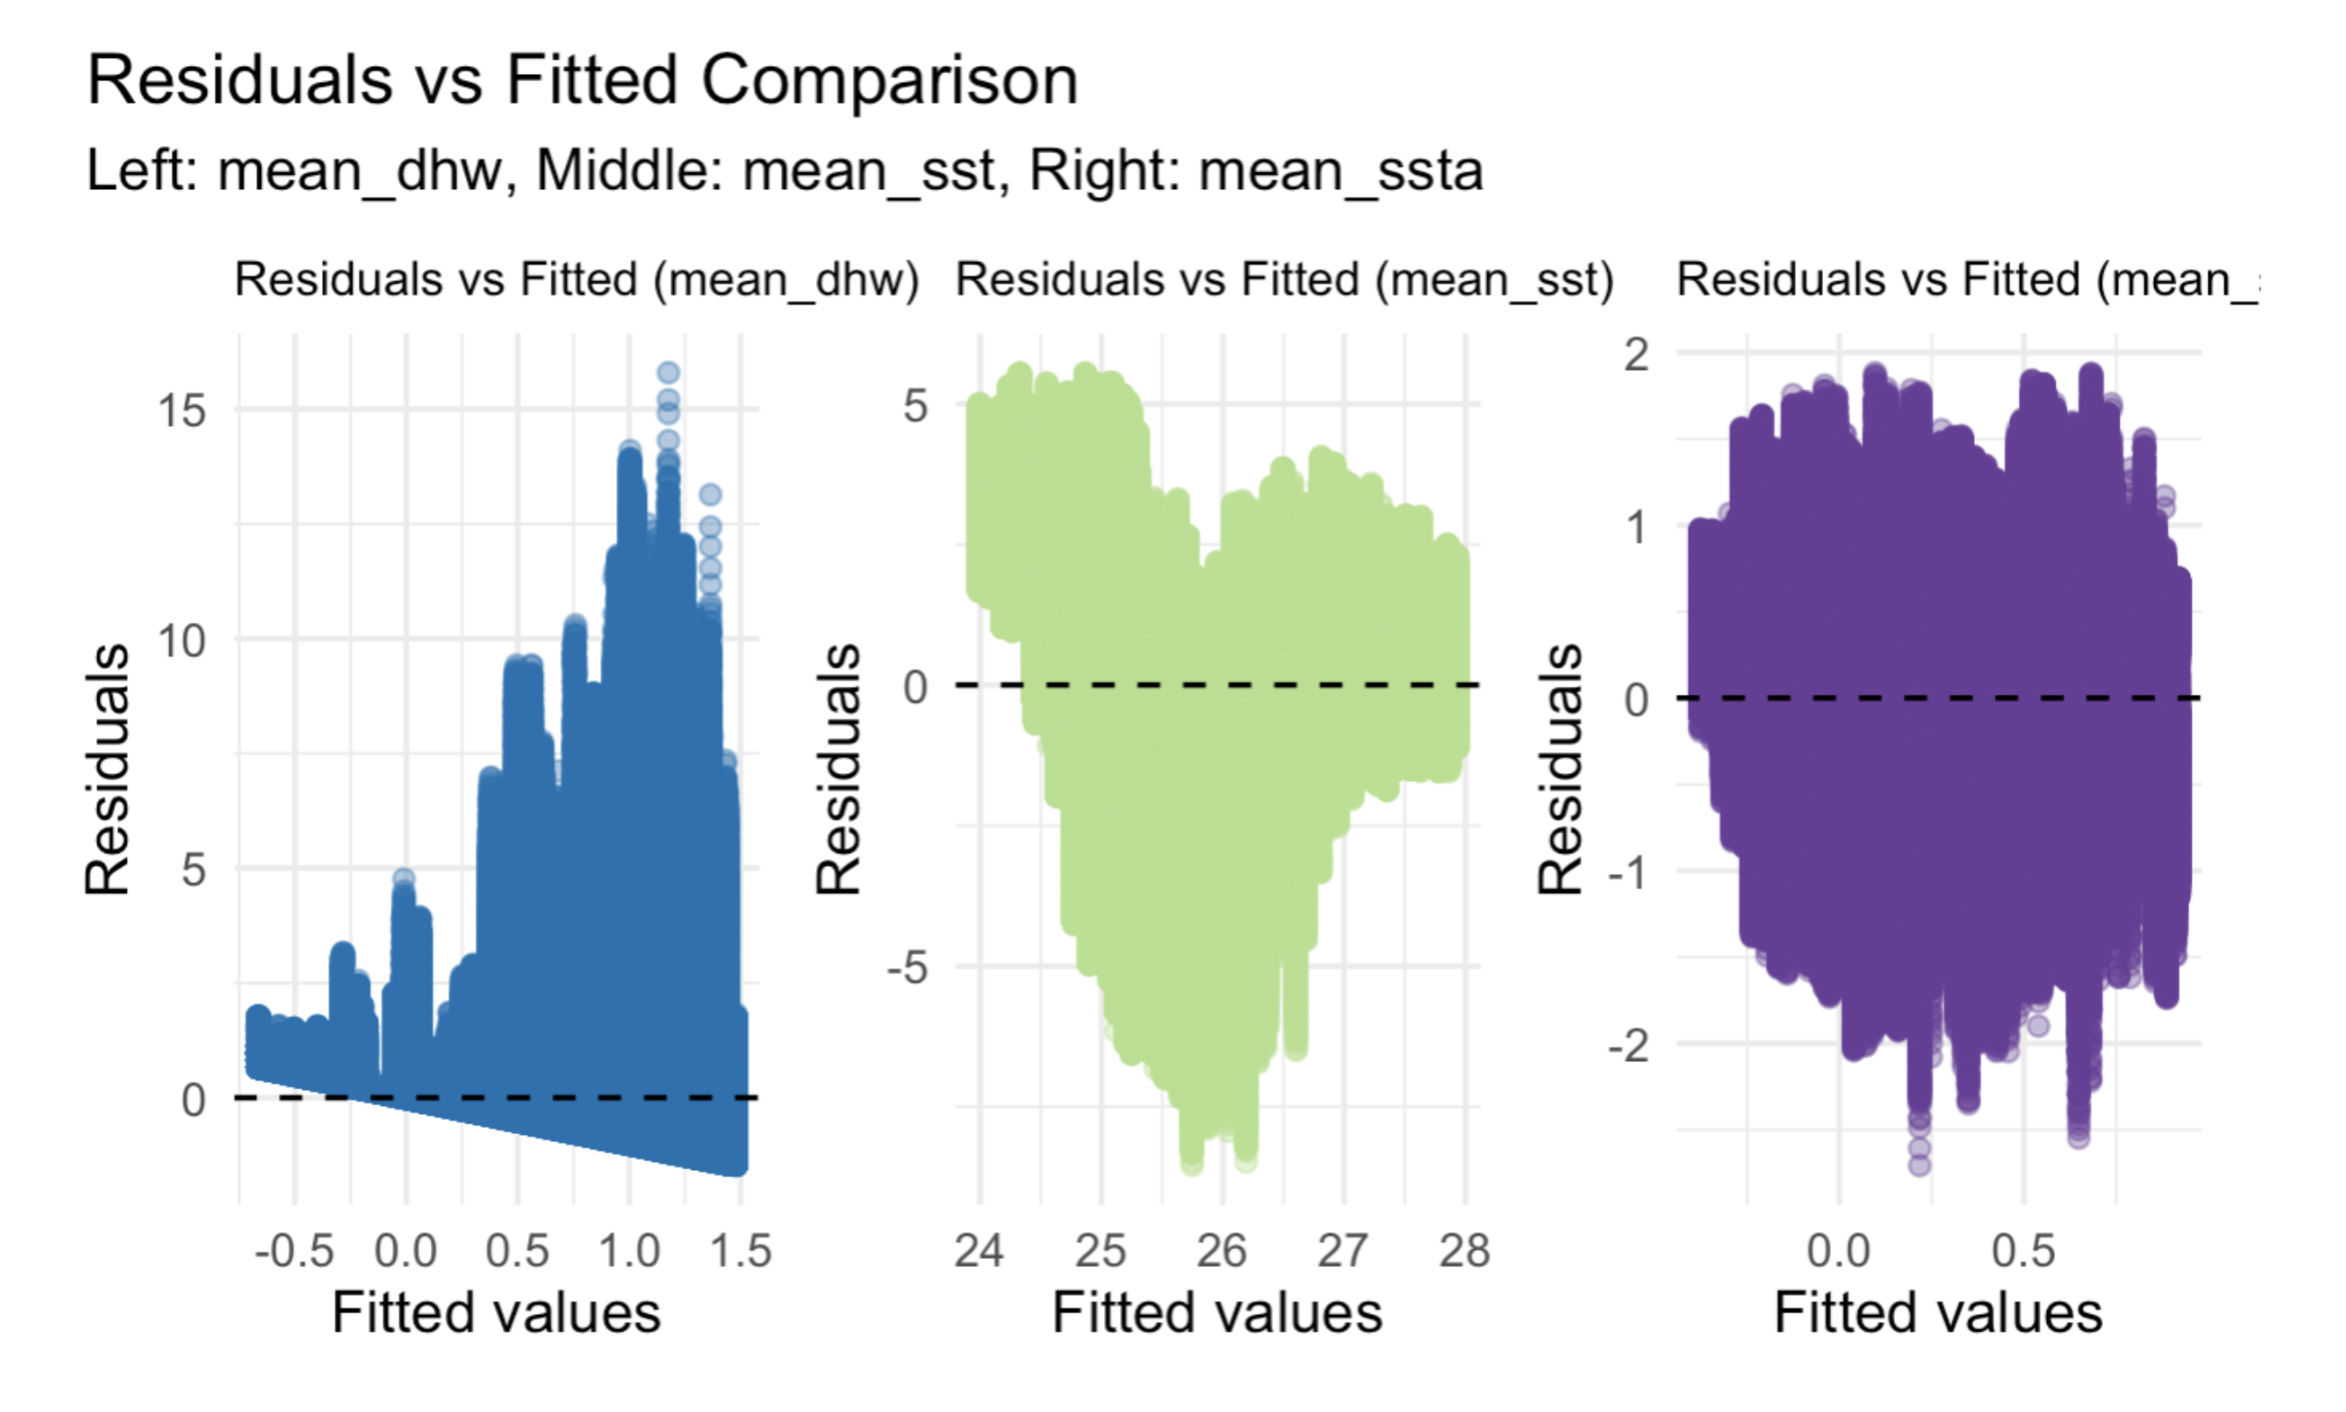
\includegraphics[width=0.5\textwidth]{report_images/lr_resplot.png}
\end{center}

\begin{center}
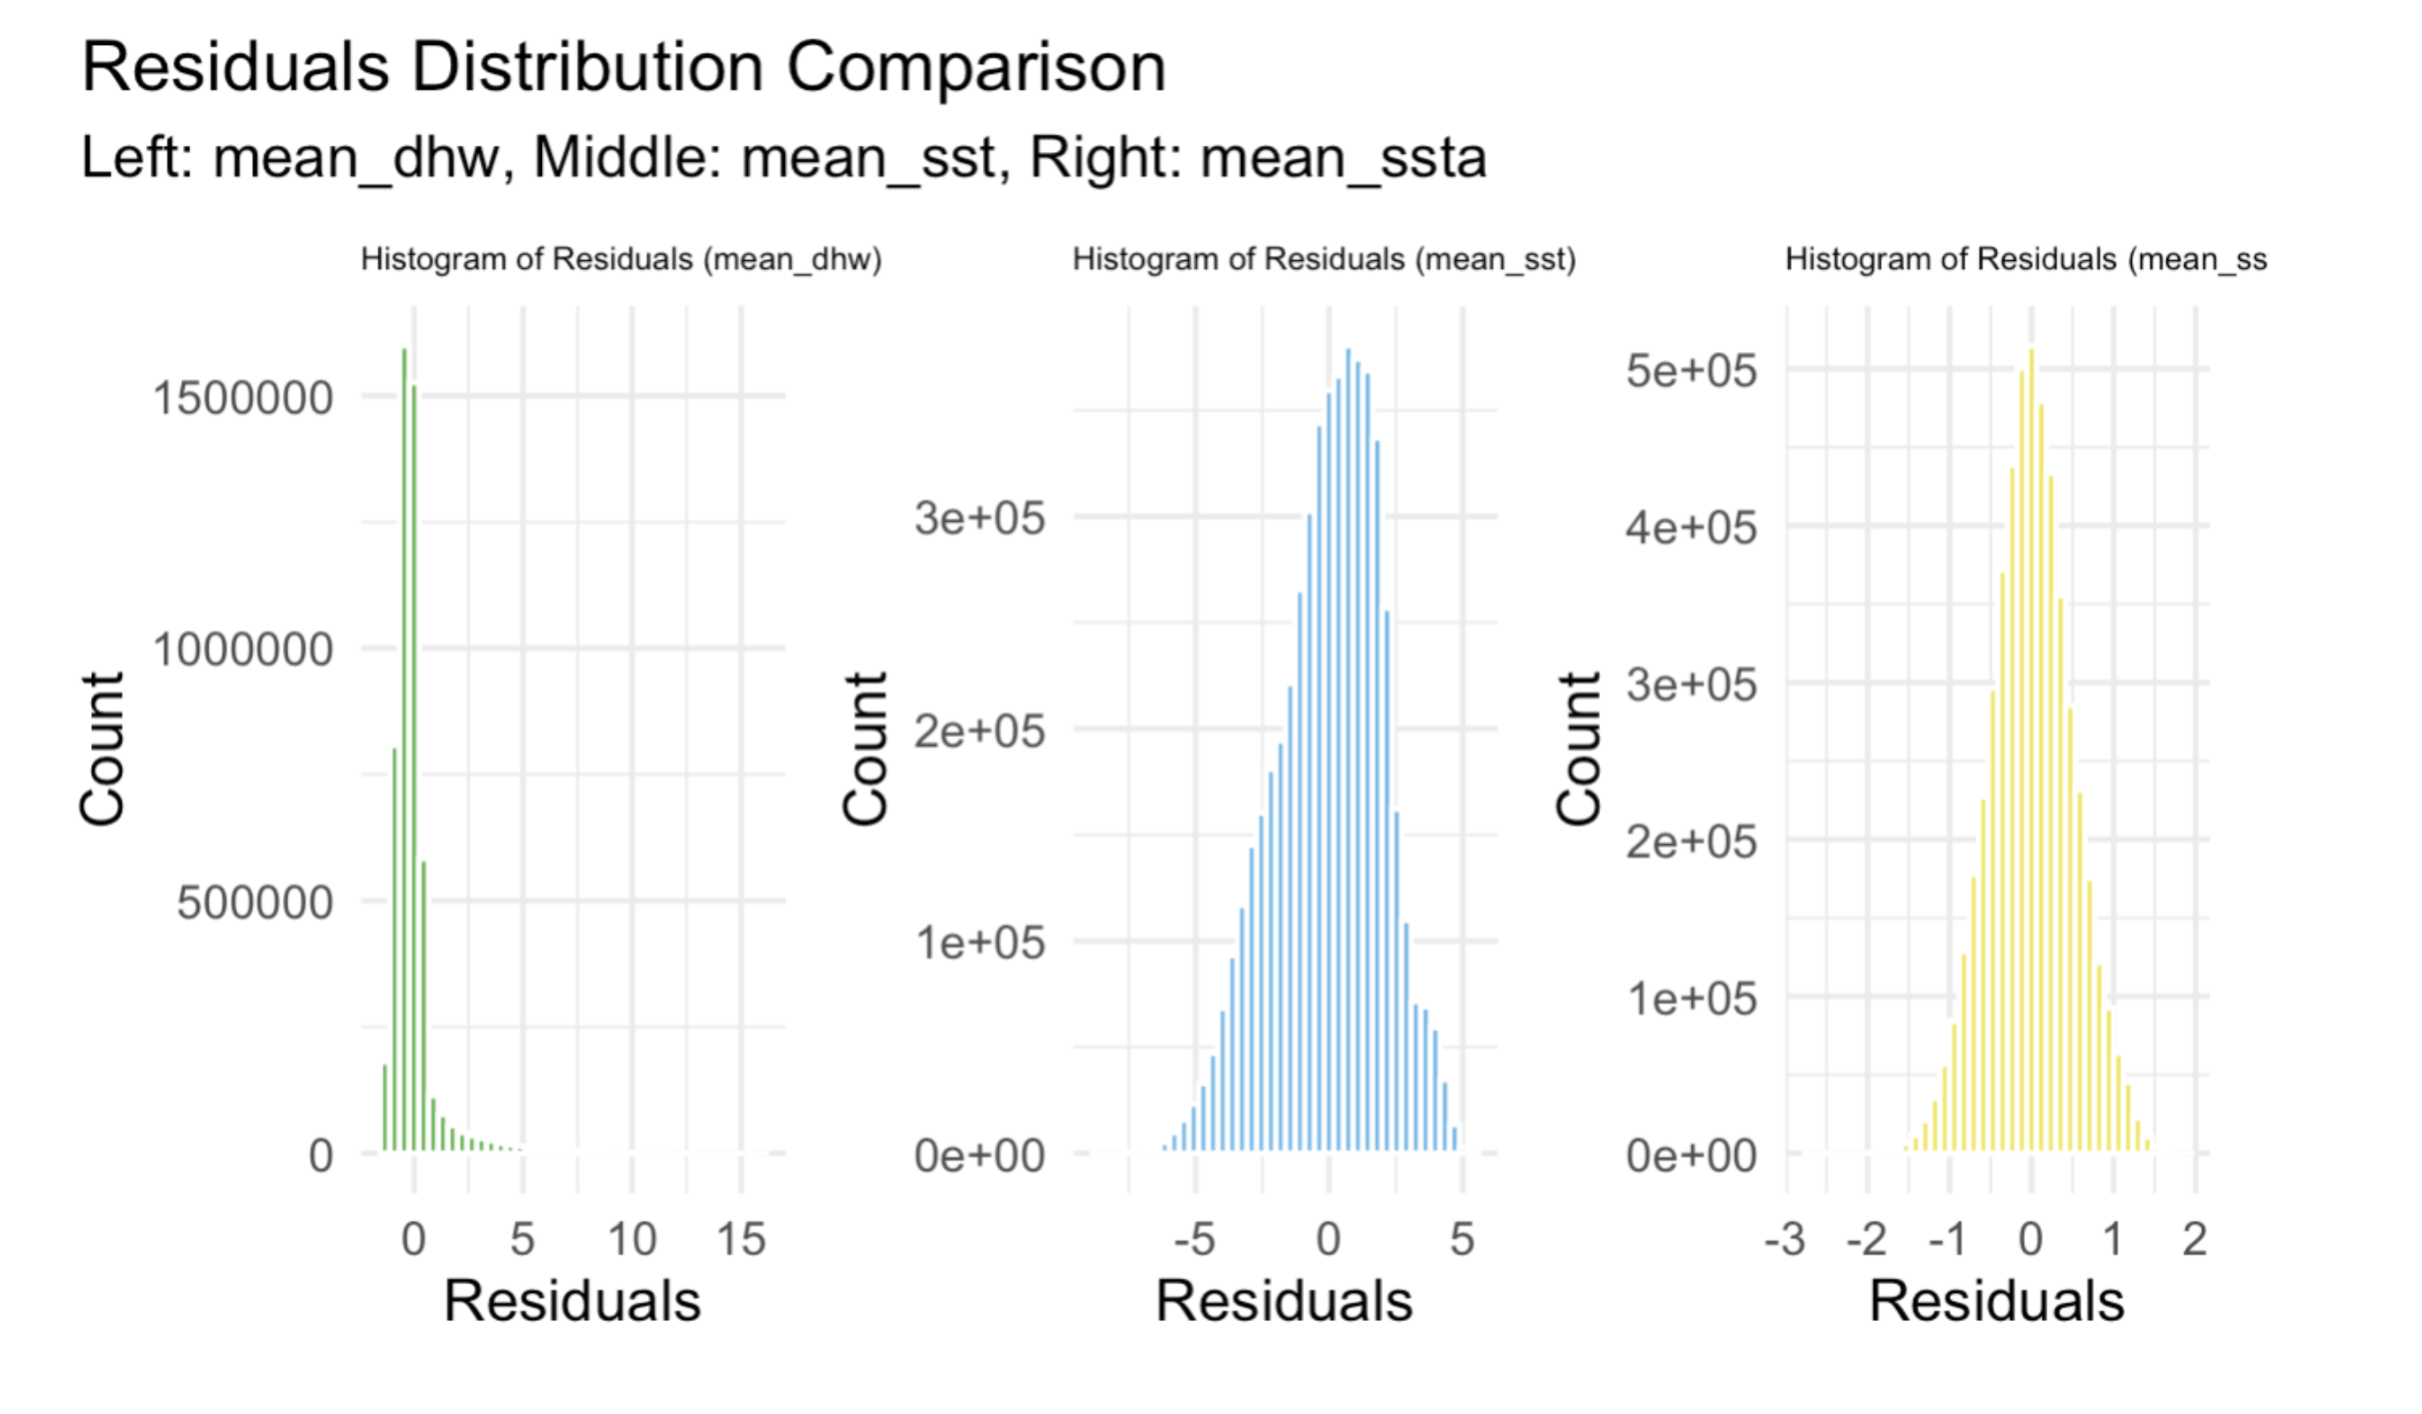
\includegraphics[width=0.5\textwidth]{report_images/lr_reshist.png}
\end{center}

\subsubsection{Appendix W: Linear Regression Predicted vs
Actual}\label{appendix-w-linear-regression-predicted-vs-actual}

\begin{center}
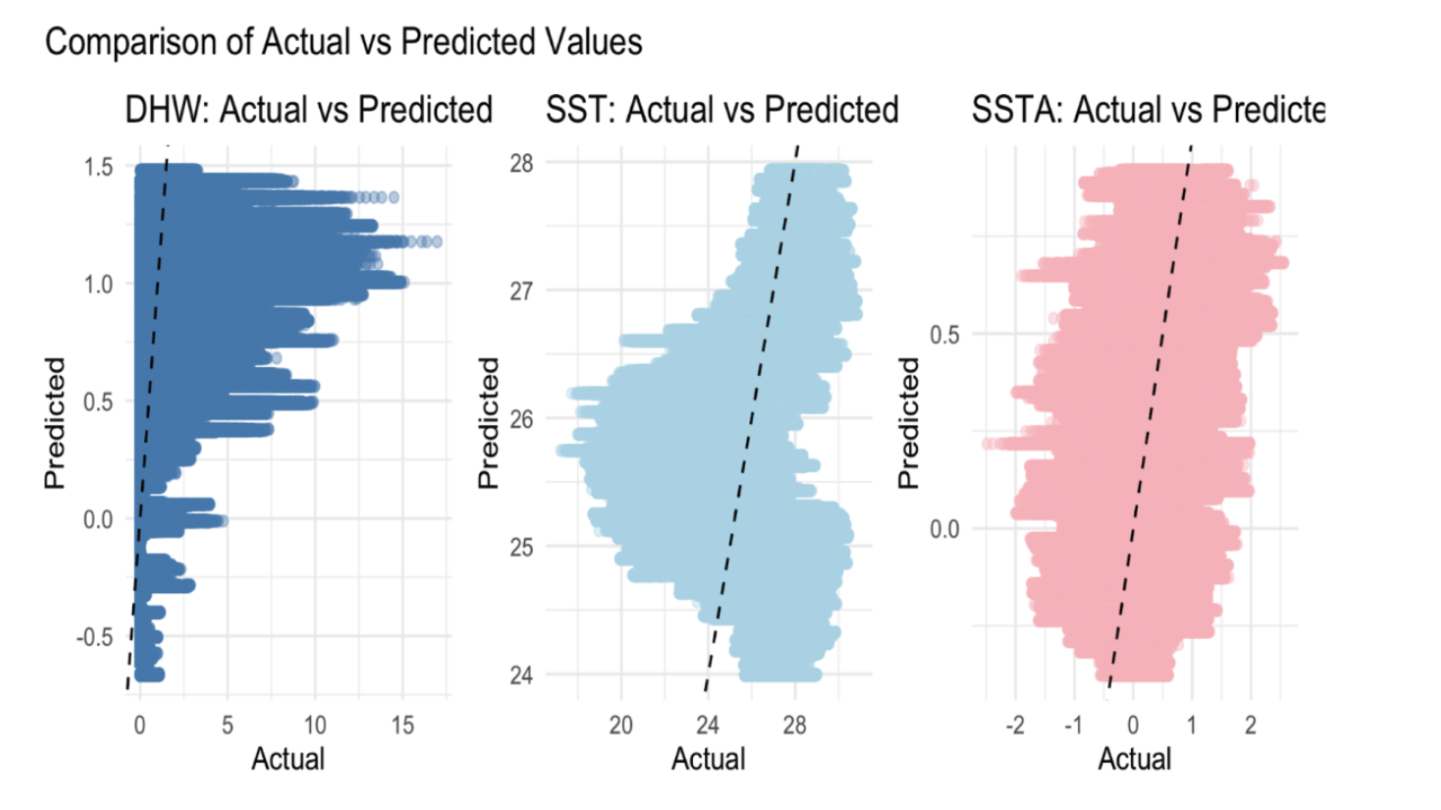
\includegraphics[width=0.5\textwidth]{report_images/lr_graph.png}
\end{center}

\subsubsection{Appendix X: Global GAM Model
Summaries}\label{appendix-x-global-gam-model-summaries}

\begin{ShadedResult}
\begin{verbatim}


Table: Smooth Terms for GAM (DHW)

|    edf|       F| p.value|term                   |
|------:|-------:|-------:|:----------------------|
|  6.867|  36.004|   0.000|s(soi_anomaly)         |
|  8.905|  66.803|   0.000|s(year)                |
|  8.177| 161.333|   0.000|s(month)               |
|  1.218|   0.733|   0.344|ti(soi_anomaly):shelfI |
|  1.001|   1.331|   0.249|ti(soi_anomaly):shelfM |
|  1.000|   1.349|   0.246|ti(soi_anomaly):shelfO |
| 15.675| 121.842|   0.000|ti(soi_anomaly,year)   |
| 76.393|  36.669|   0.000|ti(soi_anomaly,month)  |

\end{verbatim}
\end{ShadedResult}

\begin{ShadedResult}
\begin{verbatim}


Table: Smooth Terms for GAM (SST)

|    edf|       F| p.value|term                   |
|------:|-------:|-------:|:----------------------|
|  6.966|  23.320|   0.000|s(soi_anomaly)         |
|  8.957| 120.096|   0.000|s(year)                |
|  9.598| 263.824|   0.000|s(month)               |
|  1.002|   2.561|   0.109|ti(soi_anomaly):shelfI |
|  1.002|   2.353|   0.125|ti(soi_anomaly):shelfM |
|  3.561|  16.385|   0.000|ti(soi_anomaly):shelfO |
| 14.481|  19.844|   0.000|ti(soi_anomaly,year)   |
| 60.950|  14.057|   0.000|ti(soi_anomaly,month)  |

\end{verbatim}
\end{ShadedResult}

\begin{ShadedResult}
\begin{verbatim}


Table: Smooth Terms for GAM (SSTA)

|    edf|       F| p.value|term                   |
|------:|-------:|-------:|:----------------------|
|  7.419| 113.082|   0.000|s(soi_anomaly)         |
|  8.985| 405.180|   0.000|s(year)                |
|  9.775| 139.813|   0.000|s(month)               |
|  2.810|   5.806|   0.000|ti(soi_anomaly):shelfI |
|  1.000|  11.492|   0.001|ti(soi_anomaly):shelfM |
|  1.147|   8.409|   0.002|ti(soi_anomaly):shelfO |
| 15.780|  66.586|   0.000|ti(soi_anomaly,year)   |
| 89.329| 122.515|   0.000|ti(soi_anomaly,month)  |

\end{verbatim}
\end{ShadedResult}

\subsubsection{Appendix Y: Global GAM `SOI' Smoothed Functions by
`Shelf'}\label{appendix-y-global-gam-soi-smoothed-functions-by-shelf}

\begin{center}
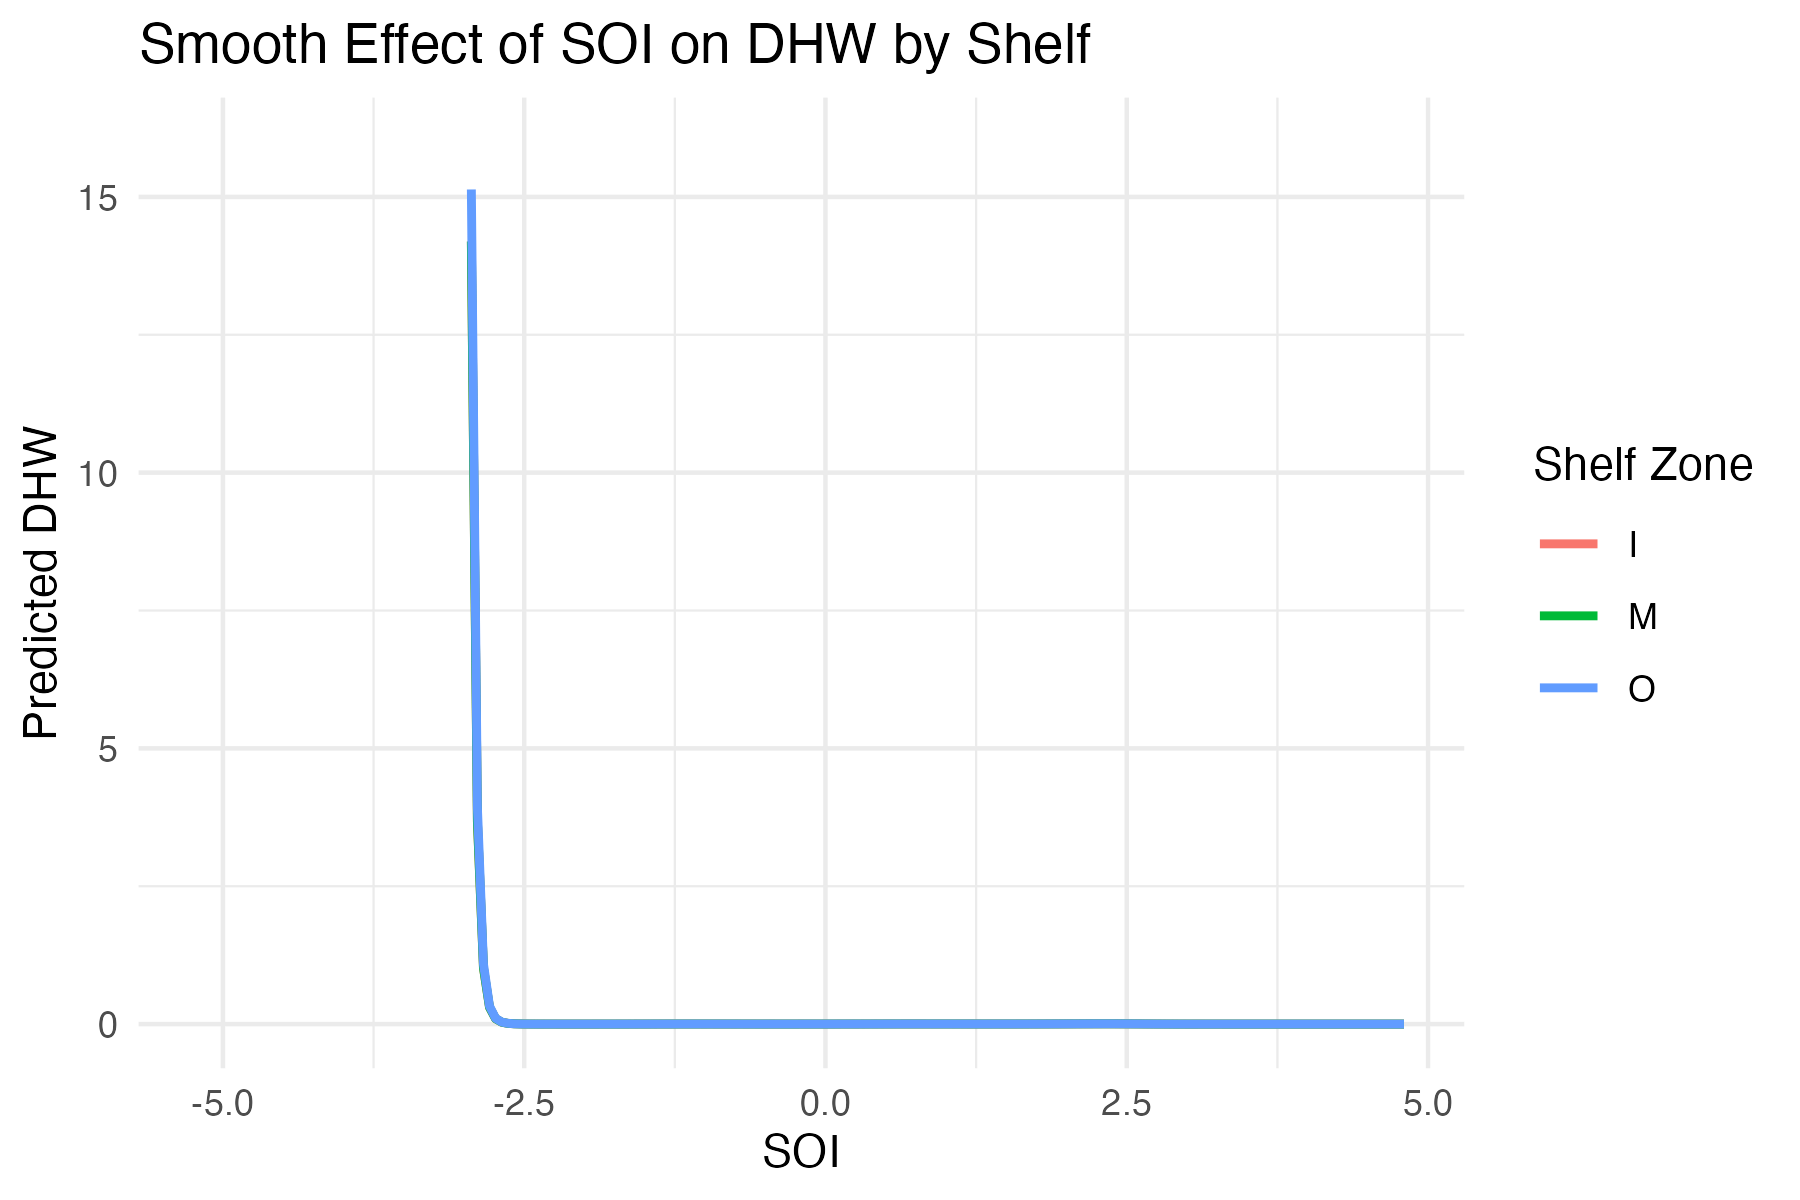
\includegraphics[width=0.5\textwidth]{report_images/soi_shelf_dhw.png}
\end{center}

\begin{center}
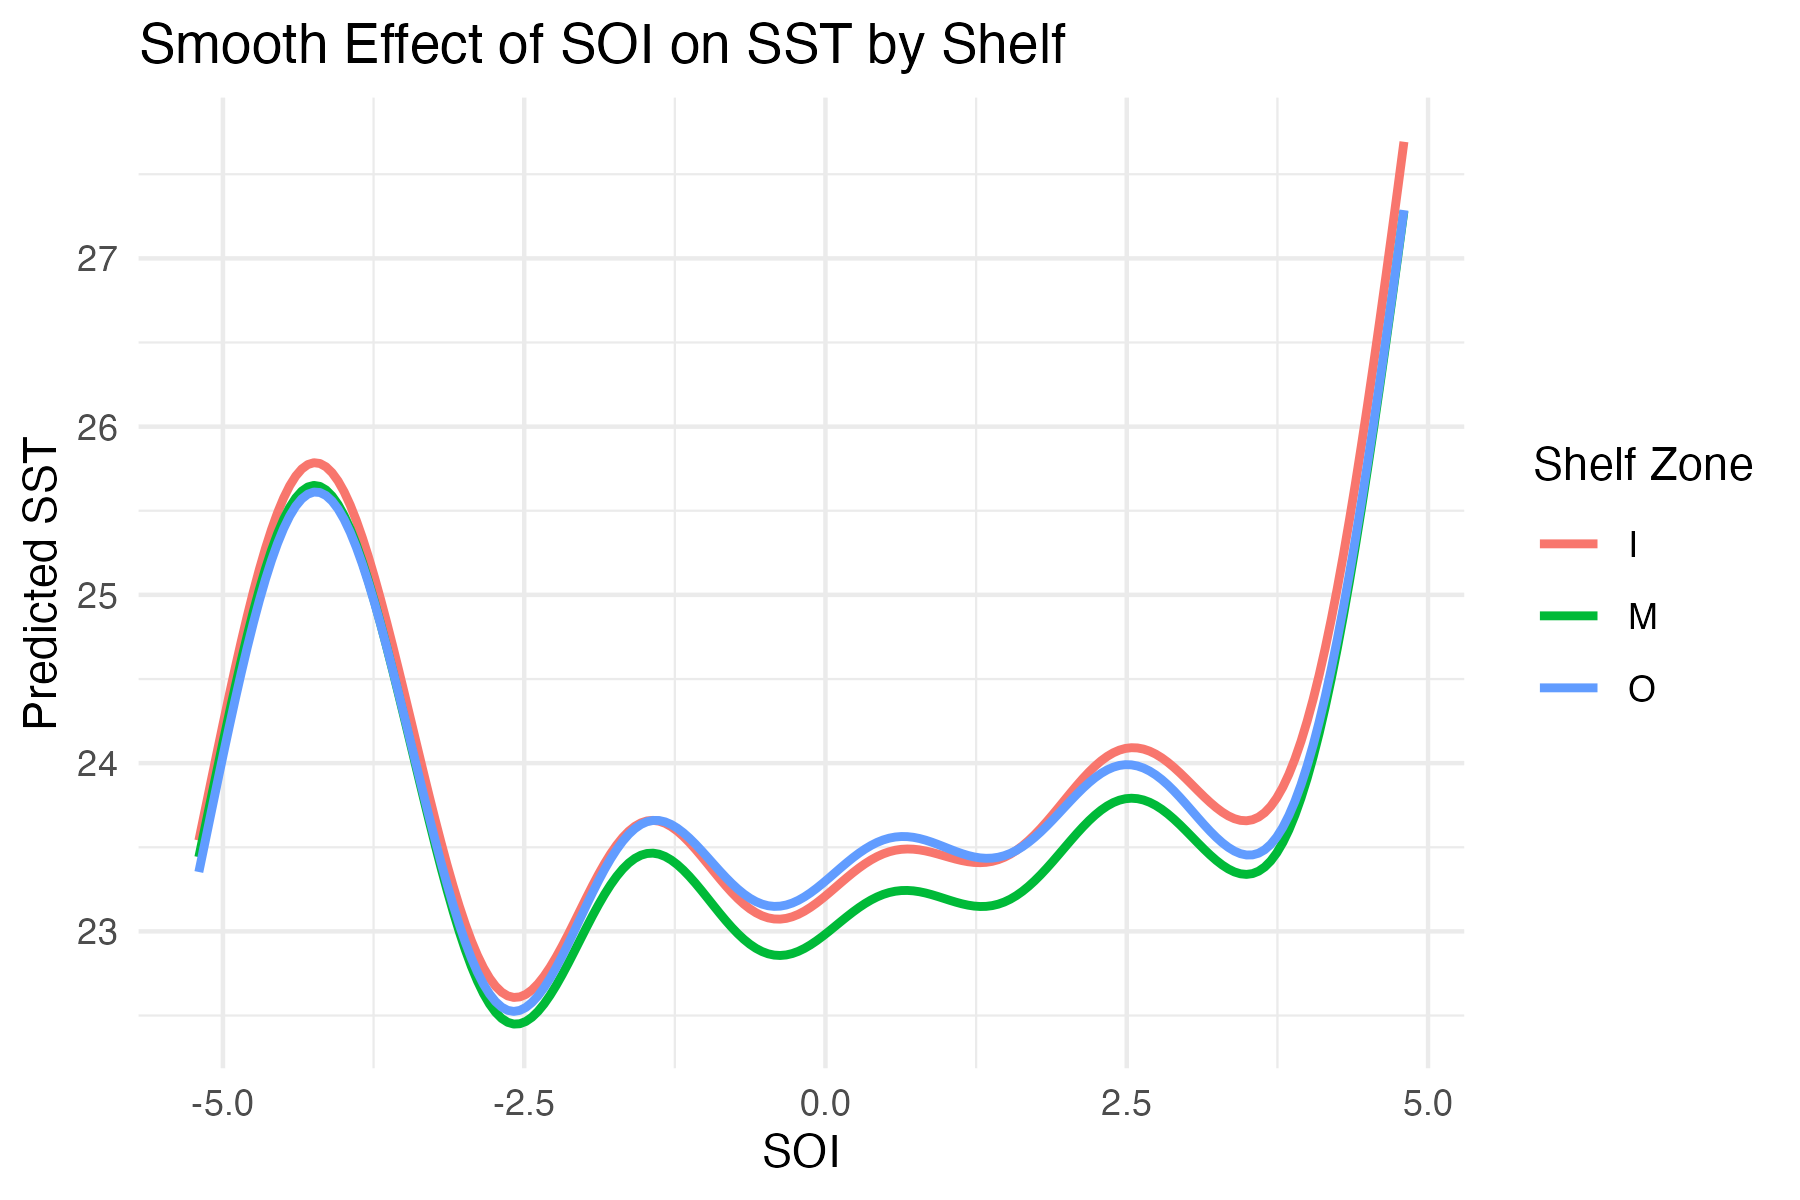
\includegraphics[width=0.5\textwidth]{report_images/soi_shelf_sst.png}
\end{center}

\begin{center}
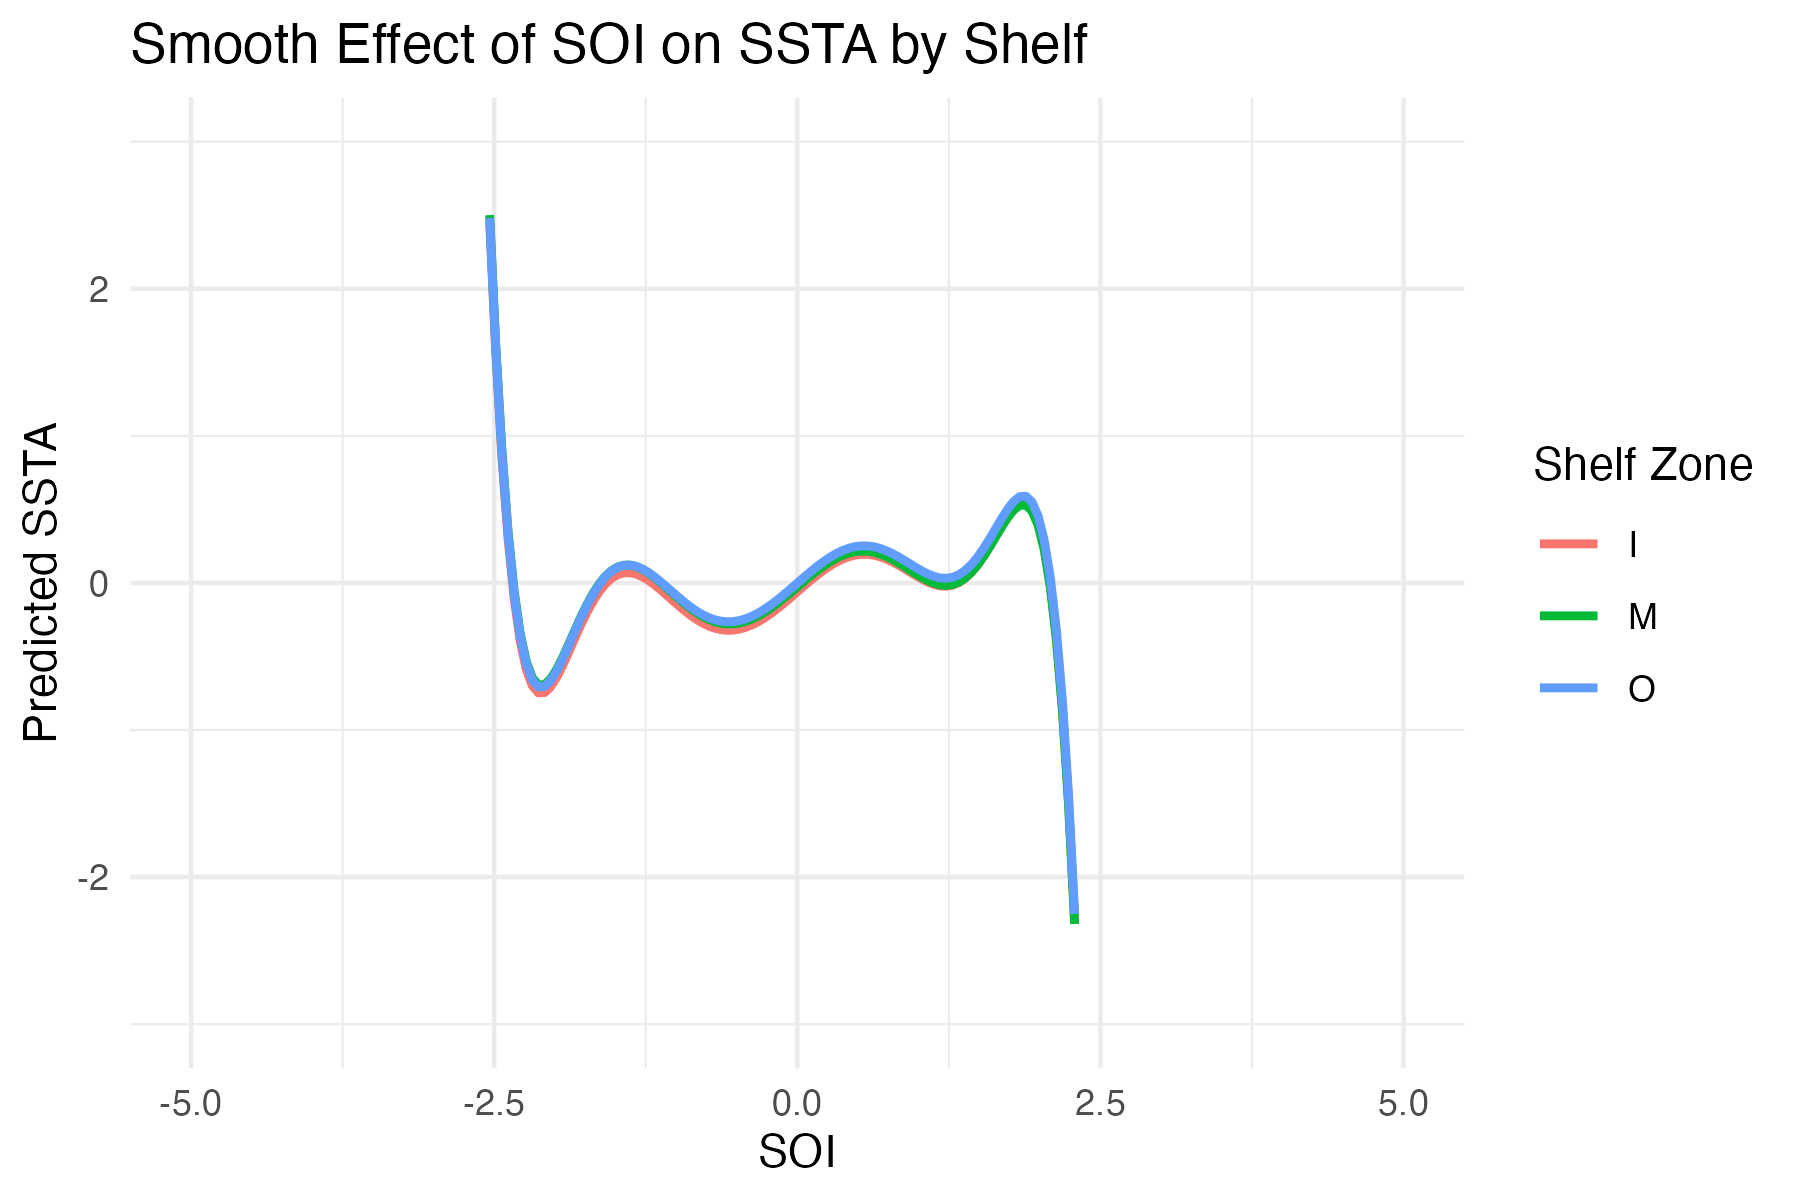
\includegraphics[width=0.5\textwidth]{report_images/soi_shelf_ssta.png}
\end{center}

\subsubsection{Appendix Z: Global GAM `SOI' Smoothed Functions by
`Month'}\label{appendix-z-global-gam-soi-smoothed-functions-by-month}

\begin{center}
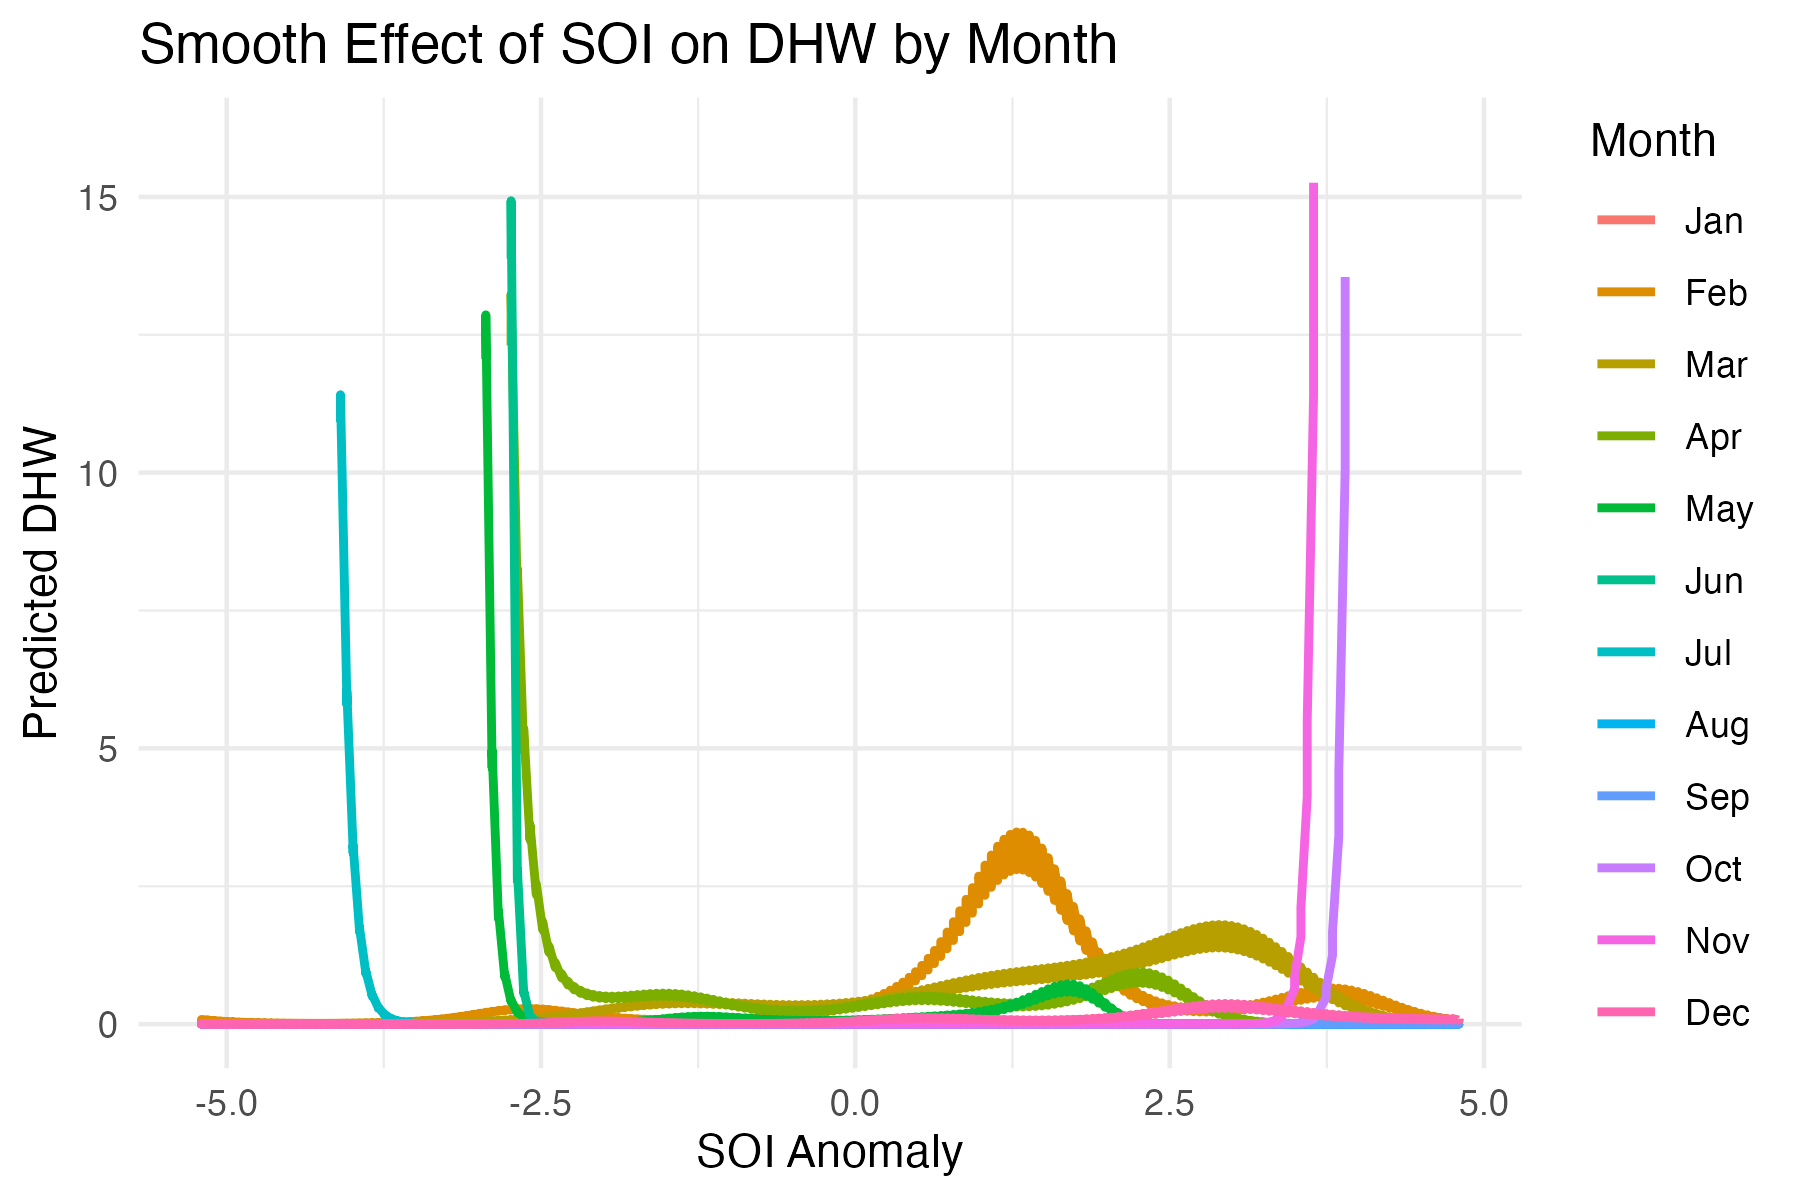
\includegraphics[width=0.5\textwidth]{report_images/soi_month_dhw.png}
\end{center}

\begin{center}
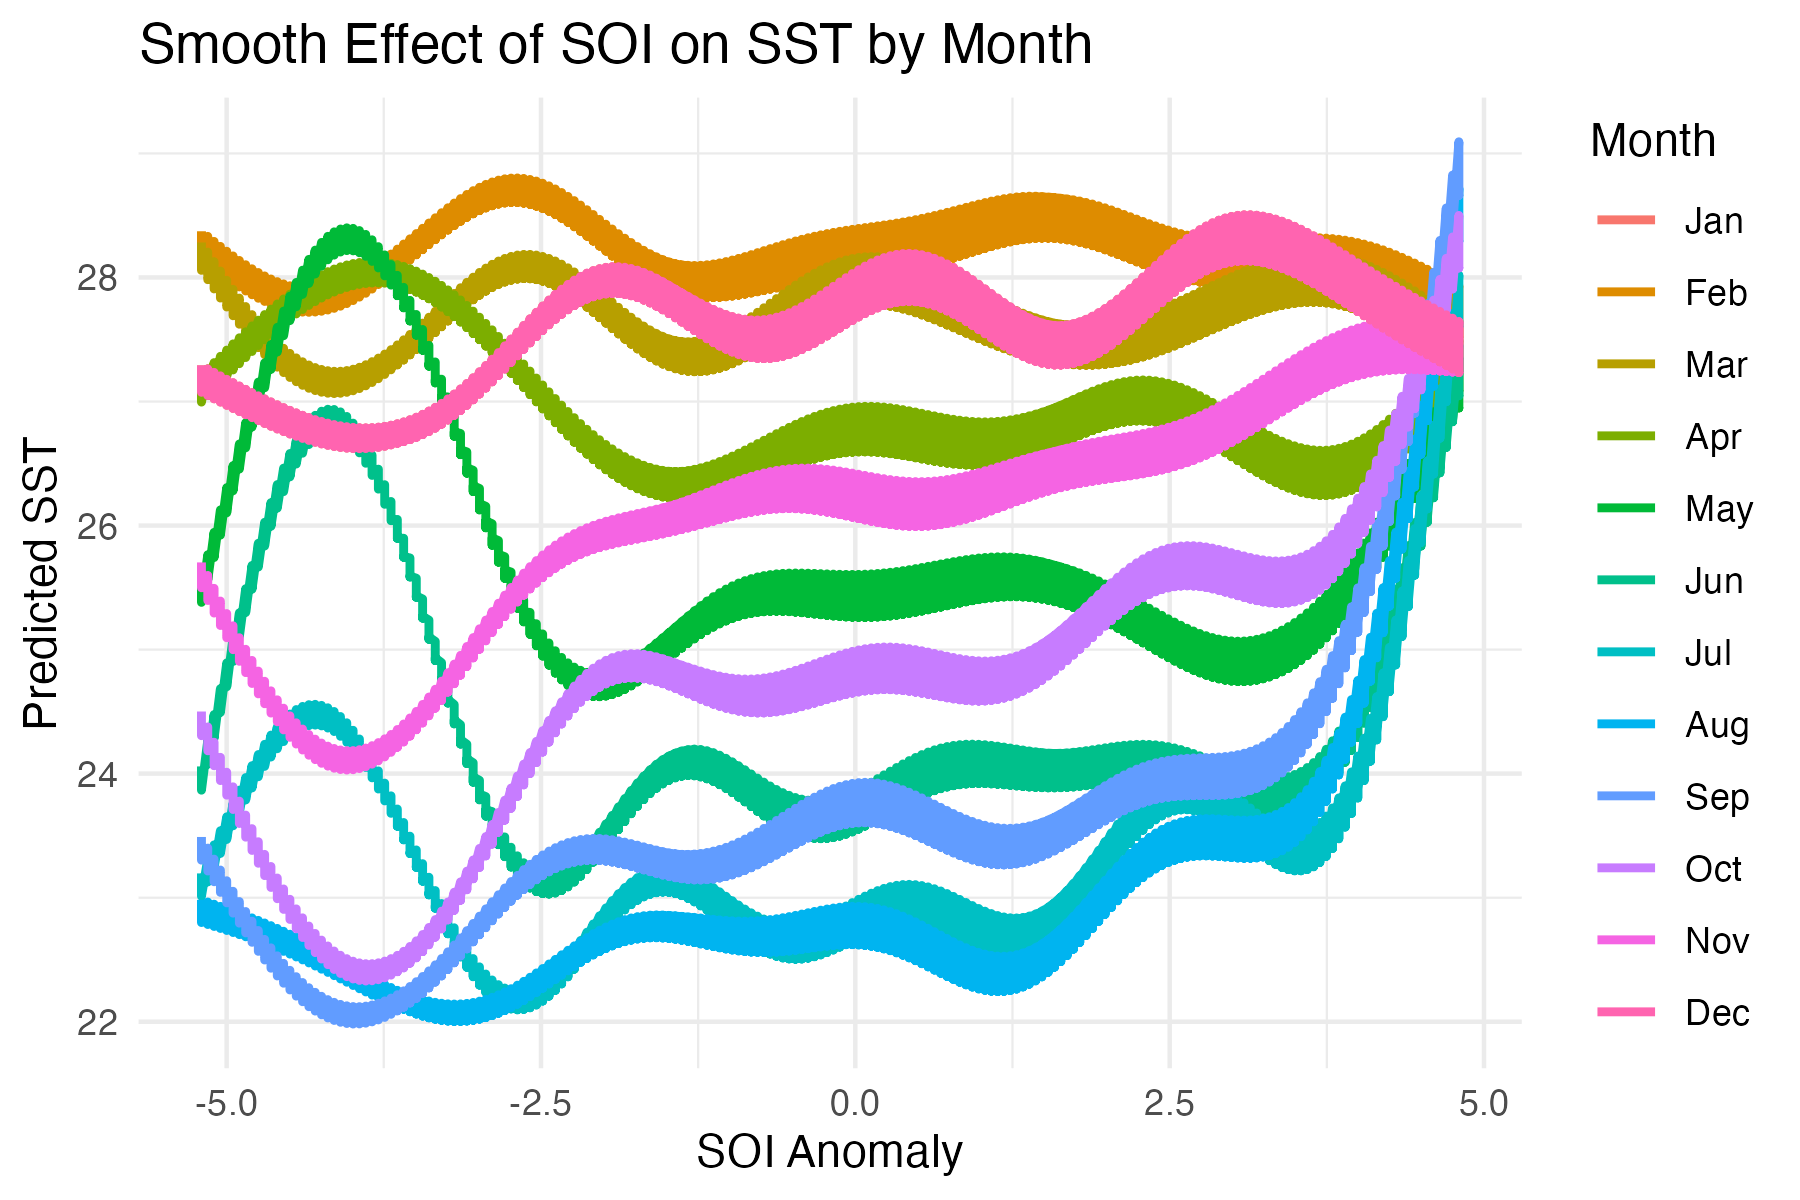
\includegraphics[width=0.5\textwidth]{report_images/soi_month_sst.png}
\end{center}

\begin{center}
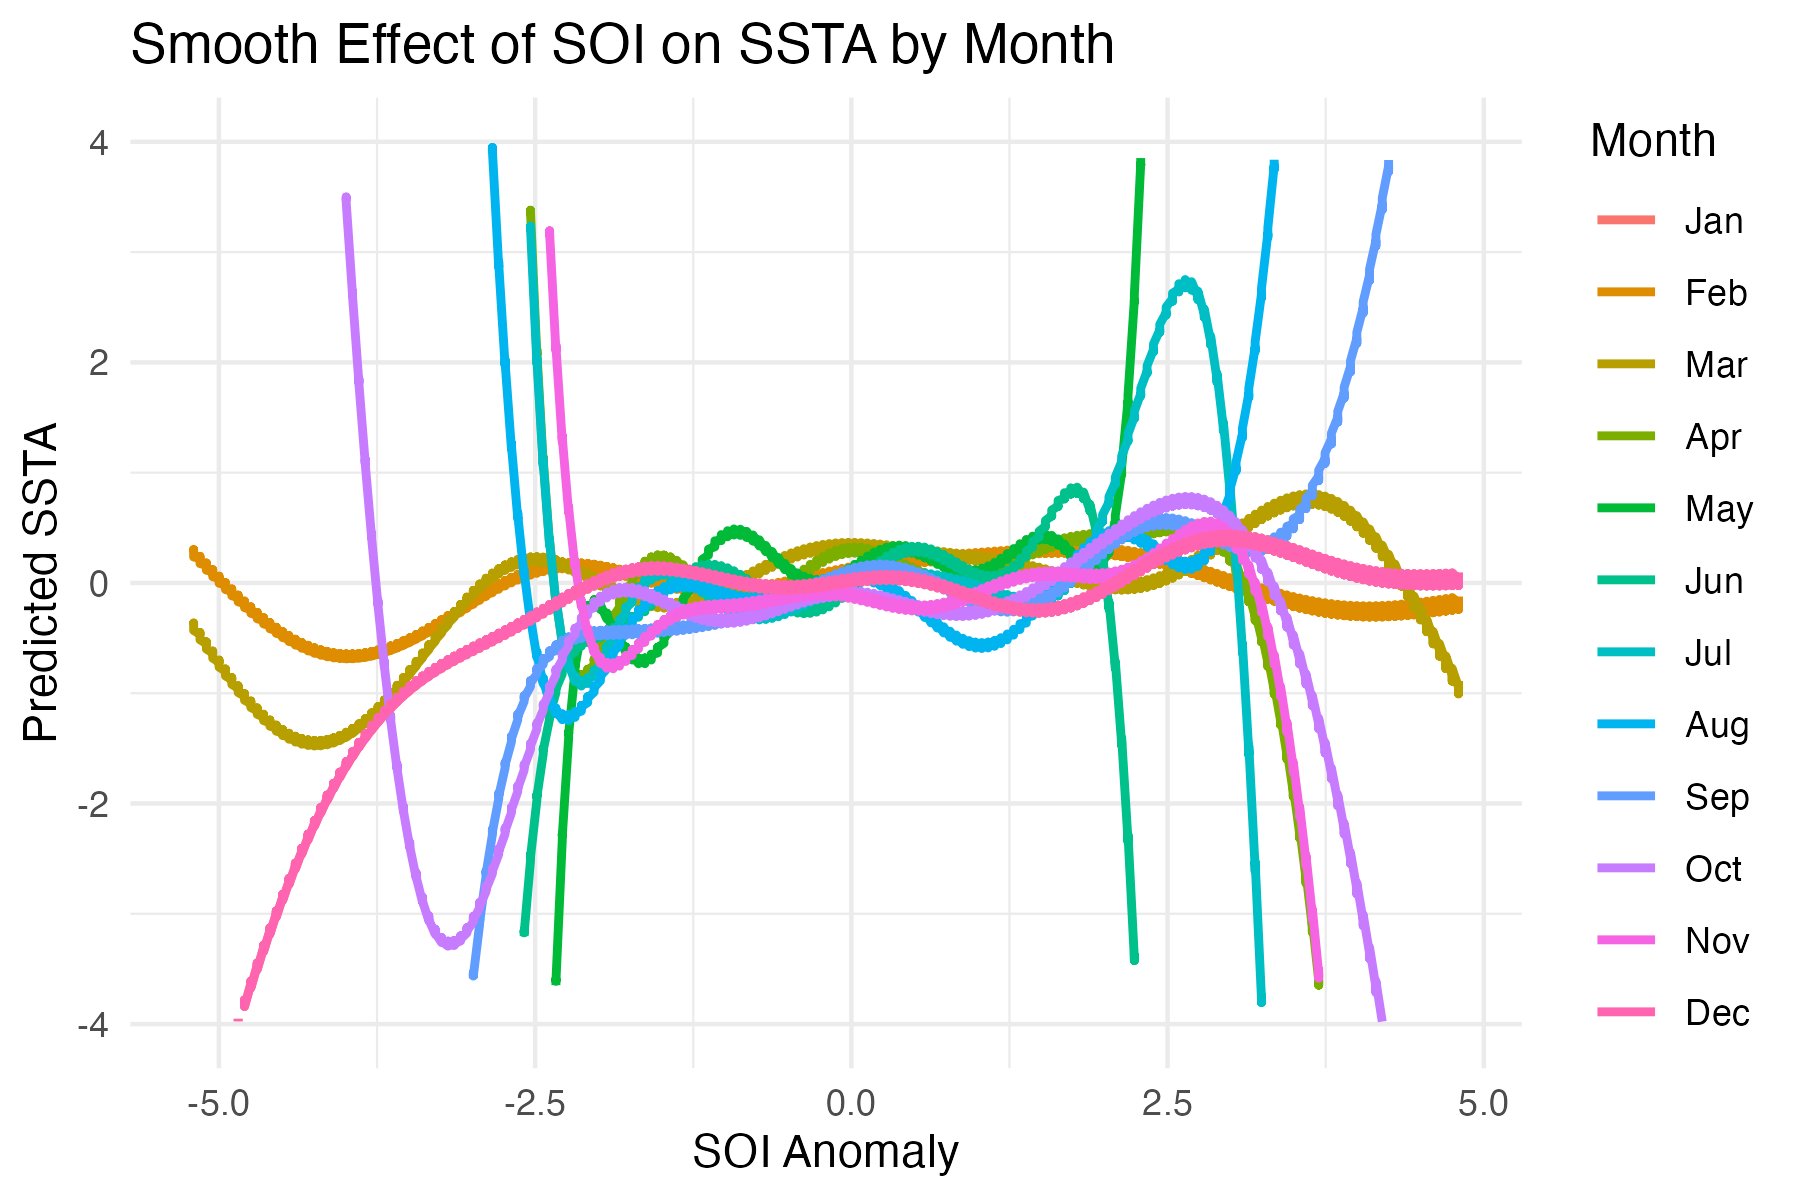
\includegraphics[width=0.5\textwidth]{report_images/soi_month_ssta.png}
\end{center}

%\showmatmethods


\bibliography{pinp}
\bibliographystyle{jss}



\end{document}
